\documentclass{eceasst}
% This is the source of the author documentation
% for the ECEASST document class.

% Required packages
% =================
\usepackage{subfig}

% Volume frontmatter
% ==================
% Volume frontmatter for OCL 2011
% =====================================
\volume{44}{2011} % Volume number and year
\volumetitle{% Title of the volume (optional)
Proceedings of the\\
Workshop on OCL and Textual Modelling\\
(OCL 2011)}
\volumeshort{% Short title of the volume (optional)
Proc.\ OCL 2011}
\guesteds{% Multiple guest editors
Jordi Cabot, Tony Clark, Manuel Clavel, Martin Gogolla}


% Article frontmatter
% ===================
\title{% Title of the article
Re-engineering Eclipse MDT/OCL for Xtext}
%\short{% Short title of the article (optional)
%Re-engineering Eclipse MDT/OCL for Xtext}
\author{% Authors and references to addresses
Edward Willink\autref{1}}
\institute{% Institutes with labels
\autlabel{1} \email{ed \_at\_ willink.me.uk}, \url{http://www.eclipse.org/modeling}\\
Eclipse Modeling Project}

\abstract{
The current tooling used for the Eclipse OCL project uses an LALR parser generator. Enhancing the tooling to support editing motivated a migration to exploit the inherently model-driven characteristics of Xtext. This paper summarizes the experiences of that migration, identifies the many benefits and discusses a few changes in implementation approach that were required. Objective performance and size comparisons between the old LALR and new Xtext approach are provided.}
\keywords{OCL, meta-model, editor, Xtext, LALR, LPG, ASG, AST, CSG, CST}

\begin{document}
\maketitle

\section{Introduction}

The Object Constraint Language (OCL)\cite{OCL} evolved, initially within the Unified Modeling Language (UML)\cite{UML}, to capture modeling constraints that were inappropriate to express graphically. It was recognized that the textual modeling expression language had utility beyond UML and so OCL 2.0 was separated out when UML 2.0 was proposed. The benefits of this separation have become clear in the last few years as OCL forms the basis for alternate modeling specifications such as the Model to Text transformation language MOFM2T\cite{MOFM2T}, and the Query/View/Transformation (QVT)\cite{QVT} Model to Model transformation languages.

The Eclipse Foundation provides a Platform and Framework for industry\footnote{All Eclipse code is made available under the Eclipse Public License (EPL) avoiding the problems that arise with the GNU Public License (GPL). The EPL Open Source license and Eclipse's IP diligence avoid Intellectual Property (IP) uncertainty.} and researchers that supports a wide variety programming activities.  In the modeling domain, the Eclipse Modeling Framework (EMF) project provides the widely used Ecore foundation. Although Ecore was originally for Java-based code generation, the use of Ecore to define meta-models has come to underlie a wide variety of different Eclipse Modeling projects. More generally Ecore is used to define its own meta-model and the Eclipse support for the UML meta-model. Many Eclipse projects endeavor to support specifications such as UML, OCL, QVT and MOFM2T defined by the Object Management Group (OMG).

The Eclipse OCL\cite{MDT/OCL} support has provided basic OCL for parsing and evaluation for many years, but this support has been primarily suitable for those keen to access it from their Java code. The advent of more powerful modeling tools, that do not require Java coding, motivates a more user friendly editing and evaluation environment for OCL within Eclipse.

A very fundamental tool for developing code in any language is a text editor with rich and semantic editing capabilities.
A first attempt at an Eclipse editor extended the generic text editor facilities, but required a substantial number of repetitive manually coded classes to capture the editing semantics, and each aspect of a rich editor required integration effort.

The next attempt used the IDE Meta-Tooling Platform (IMP)\cite{IMP}, which saved much of the repetition by providing integration with the grammar tooling. This provided most of the support for many rich editing facilities. However, IP problems prevented this editor being shipped in the Eclipse Helios\cite{Helios} release and so a rapid redevelopment was required to avoid dependence on an unreleased project.

In addition to the support for OMG specifications, Eclipse projects provide useful complementary facilities. One of the successful Eclipse incubation areas has been support for Domain-Specific Languages (DSLs), for which the Xtext\cite{TMF/Xtext} tool successfully uses little more than the language grammar to provide a fairly comprehensive editing capability that can be tailored to provide really high quality capabilities.

Although OCL is perhaps a General Purpose rather than Domain-Specific Language, the need for a rapid redevelopment motivated the use of a DSL tool.

In this paper we describe this redevelopment, and since this is a redevelopment of a real language, we are able to provide realistic contrasts between the more traditional parsing approaches and the revised approaches required by Xtext and, behind the scenes, ANTLR \cite{ANTLR}. We first review the basic parsing activities and see how the old tools supported it, then we see how Xtext provides much simpler and more powerful mechanisms that do much more. The redevelopment was not always straightforward and so we then describe areas where Xtext required a different approach to be adopted. Finally we conclude with some performance metrics contrasting the traditional and the Xtext implementations.

The code for both implementations is available as part of the Eclipse Helios release. The basic Eclipse OCL installation provides just the old approach. Installation of the optional MDT/OCL Examples provides the new Xtext editors that use the new Xtext approach\footnote{Install the {\tt Modeling} / {\tt OCL Examples and Editors} feature from the \url{http://download.eclipse.org/releases/helios/} Update site.}.

\section{Background}

Figure~\ref{fig:ParsingActivities} shows the typical parsing activities involved in converting the bytes of a file containing text in some language to the Abstract Syntax Graph (ASG)\cite{dragon} for that language.
	
\begin{figure}
  \begin{center}
    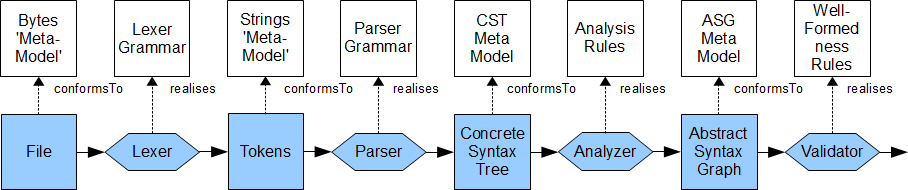
\includegraphics[width=4.75in]{ParsingPhases.png}
  \end{center}
  \caption{Parsing Activities.}
  \label{fig:ParsingActivities}
\end{figure}

Lexical analysis by a lexer combines byte sequences into tokens, then syntactic analysis in the parser establishes a hierarchical structure that is represented by a Concrete Syntax Tree (CST). For very simple languages, that can be described by an Abstract Syntax Tree (AST) rather than Graph, there may be no need for analysis to convert the CST into the ASG; CST and ASG may then be identical.  For more interesting languages, such as OCL, significant semantic analysis is required to create the ASG from the CST.

The successive representations shown as shaded squares conform to corresponding meta-models, although the first two for Bytes and Strings are perhaps too trivial to merit such a description. 

In order to appreciate the benefits of using Xtext to define a grammar (and CST), it is necessary first to present some excerpts of the more traditional LALR\cite{dragon} implementation using LPG\cite{LPG}.

Please note that for both LPG and Xtext, the examples in this paper are simplified to remove extraneous concerns.

\subsection{Basic LPG Grammar and Action Code}

An LALR grammar permits considerable precision in parsing some of the ambiguities in a grammar such as OCL. However the parse performs only syntactical analysis and so the result is a Concrete Syntax Tree that requires significant semantic analysis to create the Abstract Syntax Graph required by the OCL specification\footnote{The ASG is called an AST in the OCL specification.}.

Since the CST closely resembles the grammar, a simple BNF\cite{dragon} clause to define the grammar for a collection range such as \verb+1..10+ might be

{\small\begin{verbatim}
CollectionRangeCS ::= OclExpressionCS '..' OclExpressionCS
\end{verbatim}}

Unfortunately this has to be augmented by significant action code to populate the CST:

{\small\begin{verbatim}
CollectionRangeCS ::= OclExpressionCS '..' OclExpressionCS
  /.$BeginCode
    CollectionLiteralPartCS result = createCollectionRangeCS(
       (OCLExpressionCS)getRhsSym(1),
       (OCLExpressionCS)getRhsSym(3)
      );
     setOffsets(result, (CSTNode)getRhsSym(1), (CSTNode)getRhsSym(3));
     setResult(result);
    $EndCode
  ./
\end{verbatim}}

The action code is very repetitive with many opportunities for error.

Left recursions produce similarly repetitive code when defining the grammar for a collection literal such as the body of \verb+Sequence{1,2,3,4}+.

{\small\begin{verbatim}
 CollectionLiteralPartsCS ::= CollectionLiteralPartCS
  /.$BeginCode
     EList<CollectionLiteralPartCS> result =
                         new BasicEList<CollectionLiteralPartCS>();
     result.add((CollectionLiteralPartCS)getRhsSym(1));
     setResult(result);
    $EndCode
  ./
 CollectionLiteralPartsCS ::=
                CollectionLiteralPartsCS ',' CollectionLiteralPartCS
  /.$BeginCode
     EList<CollectionLiteralPartCS> result =
                        (EList<CollectionLiteralPartCS>)getRhsSym(1);
     result.add((CollectionLiteralPartCS)getRhsSym(3));
     setResult(result);
    $EndCode
  ./
\end{verbatim}}

While these examples are for LPG, similar overheads apply to yacc/bison, CUP, JavaCC, SableCC or ANTLR.

For LPG, manual definition of
\begin{itemize}
\item a two-part keyword and lexer grammar with action code
\item a parser grammar with substantial action code
\end{itemize}
is required and then LPG auto-generates
\begin{itemize}
\item a two-part lexer 
\item a parser.
\end{itemize}
No assistance is provided with the CST or ASG meta-models, analysis rules or well-formedness rules. Since LPG doesn't understand the CST, all aspects of the parser that interact with the CST must be contributed within the action code.

\subsection{Basic Xtext Grammar and `Action Code'}

The major innovation of Xtext is that it is model-driven, so Xtext understands the CST Meta-Model and as a result can auto-generate many additional facilities. By default, Xtext auto-generates the CST Meta-Model from the grammar, but allows an externally defined Meta-Model to be used if required.

For Xtext, manual definition of
\begin{itemize}
\item a parser grammar with CST meta-model annotations
\end{itemize}
is required and then Xtext auto-generates
\begin{itemize}
\item a lexer 
\item a CST Meta-Model
\item a parser that populates the CST
\item a pretty printer to translate the CST to the DSL
\item a rich editor that maintains the CST in its DSL representation
\item a framework for customization
\end{itemize}

So for less manual input than for LPG, Xtext provides much more auto-generated output. As will be seen in the following examples, it is not just less input, it is 80\% less input.

With Xtext, the CST for CollectionRangeCS (and also CollectionItemCS) can be generated automatically from the following 3 lines rather than the 10 above:

{\small\begin{verbatim}
CollectionLiteralPartCS:
  expressionCS=ExpCS ('..' lastExpressionCS=ExpCS)?
;
\end{verbatim}}

Here the `action code' comprises the two assignments to CST properties, as a result of which the  \verb#CollectionLiteralPartCS# in the CST meta-model class has \verb#expressionCS# and \verb#lastExpressionCS# properties.

The maintenance of lists is also simplified from 16 lines to 6. 

{\small\begin{verbatim}
CollectionLiteralExpCS:
  typeCS=CollectionTypeCS
  '{' (collectionLiteralParts+=CollectionLiteralPartCS
  (',' collectionLiteralParts+=CollectionLiteralPartCS)*)?
  '}'
;
\end{verbatim}}

Here the BNF extensions to support +,* and ? repetition are augmented by the `action' extension += for assignment to a collection property. A further ?= extension supports assignment to a boolean property.

These improvements give a significant reduction in line count for the grammar. In the Xtext version there is little redundancy and all symbols are subject to validation within the Xtext editor. In the LPG version, some symbols are not checked until Java code is compiled and many inconsistencies are only detected by run-time malfunction.

The Xtext version is therefore not only much smaller, but more thoroughly checked by tooling, and of course able to auto-generate much more functionality.

\subsection{Cross-references}

Few languages parse to pure trees; there are inevitably cross-references to accommodate the requirement for a graph. Resolution of these references is not accommodated in a traditional parser whose CST just stores the identifier sequence for a path-name such as A::B::C. Locating the model elements for A, B and C is one of the tasks performed by the semantic analyzer as it converts the identifier string in the CST to an element cross-reference in the ASG.

The simplified LPG grammar for a qualified name such as A::B::C is:

{\small\begin{verbatim}
pathNameCS ::= Identifier
...
pathNameCS ::= pathNameCS '::' Identifier
...
\end{verbatim}}        

In Xtext, the CST is actually a Concrete Syntax Graph (CSG) since it contains model element cross-references rather than strings. The graph-like relationships enable the auto-generated editor to offer many richer model-driven functionalities such as completion-assist and hyper-linking. A CSG is clearly more like an ASG than a CST is, so for some languages, it may be possible to dispense with a separate analyzer pass for CSG to ASG conversion.

Support for references is provided by the \verb+[type|token]+ syntax which parses for a lexical `token' and then performs analysis for a semantic `type'. The correspondingly simplified Xtext grammar is:

{\small\begin{verbatim}
pathNameCS returns PathNameExpCS:
  (namespace+=[Namespace|Identifier] '::')*
  element=[NamedElement|Identifier]
;
\end{verbatim}}

Here an arbitrary number of \verb+Identifier '::'+ prefixes may precede an \verb+Identifier+. The prefixes are each analyzed as \verb+Namespace+ and the \verb+PathNameExpCS::namespace+ feature accumulates them. The final \verb+Identifier+ is analyzed as a \verb+NamedElement+ and assigned to the \verb+PathNameExpCS::element+ feature.

The \verb+Namespace+ and \verb+NamedElement+ classes are part of the ASG, and their instances may be either objects created by conversion of the CSG to the ASG or objects imported from an external model. 

Xtext is able to auto-generate a default analyzer using hierarchical containment to define scoping, however most real languages have rather more sophisticated scoping and visibility rules. Xtext therefore provides a variety of techniques to support customization to solve this and other problems. For the Complete OCL grammar, these techniques are used to define the CSG to ASG manually. 

\section{Changes of Approach}

With semantic analysis integrated into the grammar, the auto-generated parser maintains a CSG that is much closer to an ASG than is traditional. This increase in capability inevitably requires that some aspects of traditional approaches need revisiting. We will therefore now describe areas where it was necessary to adopt a different approach when using Xtext.

\subsection{Left Recursion}

LALR grammars are traditionally written in left recursive style. 

{\small\begin{verbatim}
multiplicativeCS ::= unaryCS
multiplicativeCS ::= multiplicativeCS '*' unaryCS
...
multiplicativeCS ::= multiplicativeCS '/' unaryCS
...
\end{verbatim}}

A repeated term such as \verb+8/4/2+ is parsed first by reduction\footnote{The reader is referred to \cite{dragon} for a description of shift and reduce transitions.} of \verb+8+ via \verb+unaryCS+ and then via \verb+multiplicativeCS+. This is followed by reduction of \verb+4+ via \verb+unaryCS+ so that a further \verb+multiplicativeCS+ reduction gives the  \verb+multiplicativeCS+ for \verb+(8/4)+. Finally after reduction of \verb+2+ via \verb+unaryCS+, reduction of \verb+multiplicativeCS+ gives a \verb+multiplicativeCS+ for \verb+((8/4)/2)+.

This resolves precedence and associativity in accordance with typical language specifications and makes as much progress as possible with `shift' transitions along the rule before a `reduction' at the end of the rule. LALR grammars parse alternate syntax hypotheses concurrently for `shift's but require only one alternative to remain valid for the `reduction'.

ANTLR, and consequently Xtext, supports only right recursion and so the corresponding right recursive exposition in Xtext would parse \verb+8/4/2+ as \verb+8/(4/2)+ rather than \verb+(8/4)/2+. This mis-parse is predictable and so could be corrected during the CSG to ASG conversion. However Xtext's extended BNF comes to the rescue for practical use cases.

{\small\begin{verbatim}
multiplicativeCS: unaryCS (('*'|'/') unaryCS)*;
\end{verbatim}}

This extends the higher precedence \verb+unaryCS+ with an arbitrary repetition of equi-precedence terms. In detail, showing the full `action code' complexity.

{\small\begin{verbatim}
multiplicativeCS returns ExpCS:
  unaryCS
  ({InfixExpCS.source=current} op=('*'|'/') argument=unaryCS)*
;
\end{verbatim}}

The \verb+ExpCS+ return type is now non-trivial since a multiplicative expression may be one of a wide variety of alternate CSG node types. For the simple parse of just a unary expression, the \verb+unaryCS+ provides an appropriately typed term that is just `returned' unchanged. For the more interesting case where a multiplicative operator is present, a CSG node must be constructed to capture the left-operator-right context. Xtext provides special support for this, through the \verb+{}+ action clause, that first defines \verb+InfixExpCS+ as the required type of the constructed CSG node, and then assigns the left node to the \verb+source+ property from the \verb+current+ CSG context. The operator and right nodes are assigned in more obvious fashion to \verb+op+ and \verb+argument+ properties.

What could have been a significant Xtext limitation appears in practice to once again offer a significant saving compared to the LALR approach. The \verb+('*'|'/')+ and recursion save a couple of lines.

\subsection{Overlapping Syntaxes}

It is difficult to create a parser for the OCL grammar for a variety of reasons. One of these is the status of names. For instance, under what circumstances may \verb+String+,  \verb+Set+,  \verb+collect+, \verb+self+ or \verb+true+ be used as ordinary names as in: \verb+java::lang::String+, \verb+values.collect+ or \verb+myTest.true+? The OCL 2.2 specification is not clear and so implementers are forced to use intuition. The resolution of Issue 14583\cite{OCL2.3} for the OCL 2.3 specification is influenced by experience extending the Eclipse OCL implementation for re-use by QVT. Iterator names are not reserved at all, avoiding any impediment to extension with new names. \verb+self+ and \verb+true+ are totally reserved. \verb+String+ and \verb+Set+ are restricted, that is they are reserved except when qualified as in \verb+mine::Set+.

With iterator names unreserved, the parser must use lexical structure rather than a keyword to distinguish the iterator and operator call syntaxes. In simple cases such as \verb+any()+, this is impossible and so resolution must be deferred to the semantic analysis of \verb+any+.

For the more complex case of \verb+a.b(c,d+, the syntax of \verb+b+ is determined by the token following \verb+d+:
\begin{itemize}
\item \verb+a.b(c,d|e)+ is an iterator expression
\item\verb+a.b(c,d,e)+ is an operation call
\end{itemize}
This can be resolved by an LALR grammar without recourse to precedence rules, provided a `reduce' is avoided. This is awkward since for an operation call \verb+c+ and \verb+d+ may be arbitrary expressions, while for an iterator call they may be variable declarations. It is only when both take their simplest form of just a name that the ambiguity arises:
\begin{itemize}
\item \verb+a.b(c : String,d+ is obviously iterator syntax
\item \verb+a.b(c*2,d+ is obviously operation syntax.
\end{itemize}
Distinguishing an expression that is just a name from all other expressions is awkward but possible as shown by the LALR(1) grammar in the resolution of Issue 10439\cite{OCL2.3} for the OCL 2.3 specification.

This, perhaps too subtle, precision is just too hard for an Xtext (ANTLR-based) LL grammar to achieve directly. LL tools therefore provide backtracking support and by enabling backtracking in Xtext, it is then possible to parse for a more generalized operator call

{\small\begin{verbatim}
RoundBracketExpCS returns RoundBracketExpCS:
  name=NameExpCS ('@' pre?='pre')? '('
    (variable1=iteratorVariableCS
     ((',' variable2=iteratorVariableCS)
     |(';' variable2=iteratorAccumulatorCS))?
     '|')?
  (arguments+=ExpCS (',' arguments+=ExpCS)*)?
  ')'
;
\end{verbatim}}

Here iterator variables optionally precede operation arguments. The parser backtracks if its first attempt to parse iterator variables fails to terminate in a \verb+|+. The semantic analyzer is left to determine whether the name preceding the parentheses references an operator or iterator definition and whether the number and type of iterator variables and arguments are appropriate to the declaration. Since the generalized production rule allows \verb+@pre+ on any call, the semantic analyzer must also validate whether such usage is appropriate.

\subsection{Restricted Words}

A frequently asked question for Xtext is how to use of a keyword as both a reserved word and as an identifier. 

{\small\begin{verbatim}
context A::B           -- context is a keyword
self.context           -- context is an identifier
\end{verbatim}}

At first sight it appears that the use of \verb+'context'+ as a keyword in the grammar precludes the use of \verb+context+ by the \verb+ID+ terminal, since the default lexer uses \verb+ID+ only when there is nothing more specific. However Xtext augments the traditional terminal and production rules with an intermediate datatype rule that can merge terminal rules. Thus in:

{\small\begin{verbatim}
terminal ID:('a'..'z'|'A'..'Z'|'_') ('a'..'z'|'A'..'Z'|'_'|'0'..'9')*;
RestrictedKeyword:   'context' | 'package';
Identifier:           ID | RestrictedKeyword;
\end{verbatim}}
 
\noindent
\verb+ID+ is a terminal rule that defines the behavior of the auto-generated Lexer.

\verb+RestrictedKeyword+ is a datatype rule identifying a list of two grammar keywords.

\verb+Identifier+ is a further datatype rule merging the lexer terminal with the grammar list.

The remainder of the grammar can refer to \verb+Identifier+ without worrying about whether the name overlaps a distinct token.

This provides a very simple solution, but unfortunately has a very bad effect on the sizes of the generated grammar. The Complete OCL grammar has 14 keywords that need treatment in this fashion. Unfortunately only 9 can be defined this way before the generated ANTLR grammar hits the 64 kB Java method size limit. This occurs for Xtext 1.0.0. It is difficult to believe that this is a fundamental limitation of the ANTLR technology, so hopefully this problem will go away in a future release.

\subsection{Complex References}

In real languages, the type reference in a declaration such as \verb+name : type+ may be a simple name \verb+Boolean+ or constructed \verb+Tuple{name:String,values:Sequence(Real)}+. The absence of a bound on the nesting depth of Tuples and Collections leads to potentially unlimited complexity. Supporting this diversity provides a dilemma to meta-model developers. On the one hand the common use case of a simple reference is efficiently satisfied by a shared reference, while on the other hand the complex construct mandates a tree of composed objects whose root requires an owner. Identifying a suitable owner is a further dilemma.

\begin{figure}
  \begin{center}
    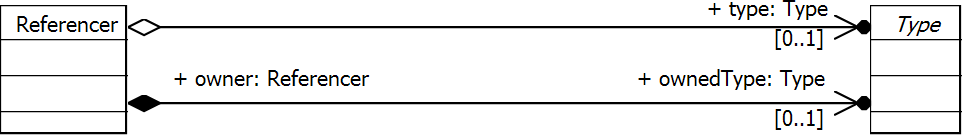
\includegraphics[width=4.75in]{SiblingReference.png}
  \end{center}
  \caption{Shared and Composed References.}
  \label{fig:SiblingReference}
\end{figure}

Figure~\ref{fig:SiblingReference} shows the simplest solution in which both a shared and a composed reference are provided but only one is used. This solution is adopted by UML for the reference from a \verb+TemplateParameterSubstitution+ to its actual parameter. Unfortunately there is always one redundant model element and common sub-trees are awkward to share.

Equivalent usages in the OCL specification omit the composed reference avoiding the redundancy but the result is that complex types just magically exist without a clear specification as to how they are persisted.

Since the meta-model representation is difficult, it is not surprising that the difficulty appears in an Xtext grammar as well. A  type reference such as \verb+type=[TypeCS|Identifier]+ in a grammar cannot accommodate a complex type. We could pursue the owned and not owned approach with \verb+(type=[TypeCS|Identifier] | ownedType=ComplexTypeCS)+, but this leaves the generated parser to resolve partial ambiguities between the two syntaxes. In practice with ANTLR technology, this means that one approach is attempted and if it fails backtracking is invoked and another alternative is attempted. At best this just costs parsing time through erroneous attempts. More of a concern arises when the first attempt succeeds because it is a prefix of the alternative; the parser then proceeds using the `wrong' parse and perhaps fails during a subsequent alternative. It is not obvious that a parser may not have a non-linear growth of backtracking alternatives to examine. With Xtext largely hiding the underlying ANTLR capabilities, it is not clear how an Xtext grammar should be written to obtain predictable and efficient results. Experience suggests that it is necessary to put more complex alternatives before simpler choices, since the complex can fail and back-track to the simple, but the converse of a false success of a simple choice does not backtrack.

The UML-style double feature approach did not appear to work well and the OCL-style magical ownership has no corresponding Xtext magic. The solution was to omit the shared reference and so treat all references as complex using \verb+ownedType=TypeRefCS+ with TypeRefCS the abstract type of a family of type reference expressions.

{\small\begin{verbatim}
TypeRefCS : SimpleTypeRefCS | ComplexTypeRefCS; // etc

SimpleTypeRefCS: type=[Type|Identifier];

ComplexTypeRefCS: type=[Type|Identifier]
       '<' ownedParams+=TypeRefCS (',' ownedParams+=TypeRefCS)* '>';
\end{verbatim}}

This approach endeavors to use an appropriate meta-model representation without redundant features. This is probably a mistake, since as shown in the simplified example above, the alternative types often share a common prefix. The parser is forced to distinguish between rather similar alternatives which may contribute to some of the adverse parsing speeds reported later. Since there is very little prospect of the CSG structure for diverse references doubling up as the ASG, it is inevitable that a slight restructuring transformation is needed between CSG and ASG. The minor aesthetic benefits of compact CSG objects is probably misguided; fewer alternatives would simplify the parser, so in the above example, \verb+SimpleTypeRefCS+ could be merged into \verb+ComplexTypeRefCS+ by making the \verb+'<' ... '>'+\footnote{Although OCL 2.2 does not support UML's templated types, OCL aspires to UML alignment. This  example is part of work to achieve alignment.} terms optional in \verb+ComplexTypeRefCS+. An LALR parser would probably mandate this change in order to eliminate a shift-reduce conflict. The Xtext tooling needs stronger diagnostic capability to advise on unwise grammar formulations. 

\section{Performance}

\subsection{Speed}

The speed of the two parsers was compared by timing the parse of an approximately 350 line Complete OCL document based on the RoyalAndLoyal example.

The first parse took 1.8 seconds with the LPG parser. 100 re-parses then averaged at 97 ms each.

The first parse took 4.8 seconds with the Xtext parser. 100 re-parses then averaged at 1114  ms each.

Comparison of the first parse time is not particularly helpful, since the measurement is quite variable, and is confounded by JVM start-up effects and the differing meta-model support. The LPG parse reads a total of two files, one for the Complete OCL document and another for the meta-model; the OCL standard library is hard coded. The Xtext parse reads six files; a file and a grammar for each of: the Complete OCL document, the Ecore meta-model and the OCL Standard Library. Since the ANTLR grammars are huge, it is perhaps surprising that the Xtext first parse is only 3 times slower.

Comparison of the re-parse times is much fairer, since the re-parses use cached meta-models and grammars. During each re-parse, LPG and Xtext parsers read just the Complete OCL document. The eleven-fold speed degradation for Xtext is disappointing but not totally surprising. Both LPG and Xtext offer opportunities for improvement, but with Xtext 1.0.0 being a very new product there are hopefully a few simple improvements that can be made before Xtext considers switching to an LALR technology.

Disclaimer: The above measurements were made using the Eclipse Helios release of Eclipse OCL (3.0.0) and Xtext (1.0.0) projects. No thorough analysis of the performance differences has been made, so the above measurements do not distinguish whether it is the Xtext parser or the MDT/OCL configuration of the Xtext parser that is slow. Informal observations suggest that there are many opportunities for caches to avoid repeated work in both projects.

The test code for these speed tests is available as an attachment to \url{https://bugs.eclipse.org/320703}.

\subsection{Grammar Size}

The example snippets above suggest that Xtext provides a three-fold reduction in grammar size.

When a full grammar is considered, the line count savings are more substantial, although there is always some uncertainty in terms of exactly what constitutes a line. The figures that follow are raw line count and so include every blank line and copyright notice, but since both sets of files use similar editorial styles, the comparative values should not differ greatly from an alternate metric based on information lines.

The entire Essential OCL grammar (both parser and lexer) requires a single 395 line Xtext file; no further template or library files are re-used.

The corresponding LPG support requires a 1485 line parser grammar, a 100 line lexer grammar and a 151 line keyword grammar. The parser extends a 785 line Java class with a further 255 lines for a lexer class. The grammars rely on nearly 1000 lines of re-usable imported templates.

It seems reasonable to summarize these figures as an at least 5-fold reduction in line count by using an Xtext grammar.

\subsection{Parser Size}

For the Complete OCL grammar, the LPG grammars produce three Java files for each the keyword, lexer and parser grammars; the total file size of all the parsing class files is 221 kB. This excludes the size of the semantic analyzer.

The Xtext auto-generates ANTLR grammars from which ANTLR generates many classes. After eliminating classes whose functionality supports semantic analysis, the total size of the class files is 2370 kB.

The Xtext parsers are therefore approximately ten times larger than their LPG counterparts.

And unfortunately the editor does not re-use this grammar. The editor support involves a further 1 MB grammar.

\section{Further Work}

\subsection{OCL re-use}

The OCL specification re-uses OCL to define constraints
\begin{itemize}
\item disambiguation rules while constructing the CST, 
\item name lookup and environment propagation within the CST, 
\item ASG construction from the CST, 
\item well-formedness rules for the ASG, 
\item well-formedness rules for evaluations using ASG
\end{itemize}

Anyone who studies these OCL constraints soon realizes that the constraints have never been subjected to a tool that provides syntactic, let alone semantic, checking. With so many basic lexical errors, what prospect is there that the constraints actually express the required functionality?

The Eclipse OCL realization of these constraints is distributed throughout the LPG parser, analyzer and validator as hand-coded Java making it difficult to determine the correspondence with the specification, even if the specification was accurate.

The Xtext re-engineering has hand-coded scoping classes that bear a superficial resemblance to the `Inherited Attributes' specifications and, as yet, no realization of the well-formedness rules at all.

For the well-formedness rules, performance concerns seem the only deterrent to a validation implementation that directly executes the OCL constraints expressed in OCL. Once the OCL specification is corrected to express the true intent, this would immediately demonstrate equivalence with the OCL specification.

The performance concerns can be mitigated by an OCL code generator of modest quality and eventually removed by a high quality OCL to Java code generator.

Referring back to Figure~\ref{fig:ParsingActivities}, we have lexer and parser grammars, analysis and well-formedness rules defined in the OCL specification. The OCL specification is moving towards providing a more usable grammar that could be more obviously equivalent to the Xtext exposition. If the OCL constraints defining the rules are used directly, we should get quite close to having OCL tooling fully defined in the specification in ways that are directly consumable by practical tooling. This should then ensure that the OCL present in the OCL specification accurately reflects the true requirements.

\subsection{Model-driven Operators}

Clause 9.3 of the OCL specification defines just the mapping of expression terms and operators from the CST to the ASG. Precedence is separately specified as a bulleted operator list and associativity is currently unspecified. This is discouraging to any implementer familiar with a grammar such as those for Java or C where precedence is integral to the grammar.

The OCL 2.2 specification resolved a precedence surprise whereby OCL 2.0 had equal precedences for \verb+and+, \verb+or+ and \verb+xor+, at the expense of introducing a compatibility surprise. An OCL tool may therefore want to provide users with a compatibility option. and more generally may want to allow addition of user-defined operators with user-defined precedences and associativity.

Perhaps the grammar could be generalized

{\small\begin{verbatim}
binaryExpression : unaryExpression (infixOperator unaryExpression)*;
unaryExpression : prefixOperator* atomicExpression;
\end{verbatim}}
 
The definitions of infixOperator could be provided as part of a customizable OCL `Standard' Library model rather than being built-in to the parser. Xtext of course makes development of a further editor for the OCL `Standard' Library quite easy.

\subsection{LPG Compatibility}

Unless Xtext is able to come close to LPG speed, the Eclipse OCL project has no alternative but to support two parsers; an LPG parser for speed and an Xtext parser for use in interactive environments such as editors. The Eclipse OCL project also has a compatibility obligation to its consumers, so the LPG interface cannot easily be discontinued.

Maintenance of two independent parsers and analyzers is not an attractive prospect. Xtext uses Xtext to define its own editor and grammar, so it should be possible to perform a Model to Model and then a Model to Text transformation on the Xtext grammar for OCL and thereby auto-generate an LPG grammar with auto-generated action code to maintain a very similar CSG model.

This should give an Xtext-defined LPG grammar avoiding the adverse performance of the ANTLR tooling and preserving the general principles of the existing parser and analyzer interface. Re-expression of the Xtext grammar in LALR form may also provide the missing diagnostics of unwise parser constructs.

\section{Conclusions}

Re-engineering the Eclipse OCL support to use Xtext 1.0.0 rather than LPG 2.0.17 has demonstrated many of the powerful benefits that Xtext offers. Subjectively Xtext is much better for common functionality and incomparably better because of the  richer tooling and extra auto-generated functionality.

Objectively, the Xtext version of the OCL grammar is at least 5 times smaller, but the generated parser is 10 times larger and 11 times slower.

It is hoped that future releases of Xtext can make significant reductions to the adverse comparisons.

Migration of LALR grammars to Xtext required re-examination of the parsing approach and some policy changes that were perhaps merited anyway.

Xtext provides good diagnosis of syntactical and simple semantic errors in an Xtext grammar. It is not clear that Xtext provides adequate diagnosis of the unexpected results that may arise through the use of backtracking.

With the aid of Xtext and other modern tooling it may be practical to have OCL editor and parser tooling reusing the exposition of grammars and constraints in the OCL specification.

%\subsection{Manual Assembly of Bibliographies}\label{bibman}

%\noindent\textbf{To Do}

\begin{acknowledge}
Many thanks to Sebastian Zarnekow, Adolfo S\'anchez-Barbudo Herrera and the anonymous reviewers for helpful comments on earlier versions of this paper.
\end{acknowledge}

\nocite{*}
\bibliographystyle{eceasst}
\bibliography{oclxtext}

\end{document}
